\documentclass[conference]{IEEEtran}
\IEEEoverridecommandlockouts
%Template version as of 6/27/2024

\usepackage[hidelinks]{hyperref}
\usepackage{cite}
\usepackage{amsmath,amssymb,amsfonts}
\usepackage{algorithmic}
\usepackage{algorithm}
\usepackage{graphicx}
\usepackage{textcomp}
\usepackage{xcolor}
\usepackage{multirow}
\usepackage{booktabs}
\def\BibTeX{{\rm B\kern-.05em{\sc i\kern-.025em b}\kern-.08em
    T\kern-.1667em\lower.7ex\hbox{E}\kern-.125emX}}
\def\IEEEkeywordsname{Keywords}
\begin{document}

\title{Counterfactual Simulation of Extreme Mental Health Scenarios for Clinical Preparedness via Fine-Tuned LLMs and Explainable AI}

\author{
\begin{tabular}{ccc}
{Gangavarapu Lakshmi Dhatri} & {Kumari Khushi Singh} & {Likitha C} \\
\textit{Dept. of CSE, REVA University} & \textit{Dept. of CSE, REVA University} & \textit{Dept. of CSE, REVA University} \\
Bengaluru, India & Bengaluru, India & Bengaluru, India \\
lakshmidhatri.gangavarapu@gmail.com & kumari.khushi.singh@gmail.com & likithaanuchandru@gmail.com \\
\end{tabular}

\\
\\

\begin{tabular}{cc}
{Harshitha N} & {Dr. Priyanka Bharti} \\
\textit{Dept. of CSE, REVA University} & \textit{Dept. of CSE, REVA University} \\
Bengaluru, India & Bengaluru, India \\
harshithamurthy31@gmail.com & priyanka.bharti@reva.edu.in \\
\end{tabular}
}

\maketitle

\begin{abstract}
Mental health crisis events including suicide attempts, psychotic breaks, and substance-induced decompensation often exhibit warning signs in clinical notes days or weeks prior, yet clinicians lack systematic tools to project potential adverse trajectories. Current AI systems focus on binary risk classification, failing to answer the critical question: ``If this patient deteriorates, what would that trajectory look like?'' This study aimed to develop an explainable counterfactual reasoning framework that generates plausible extreme mental health scenarios grounded in clinical evidence. We proposed a multi-stage pipeline comprising a fine-tuned large language model for clinical factor extraction, negation-aware safety signal detection, evidence-based scenario gating, Tree-of-Thoughts reasoning for parallel scenario generation, and post-hoc evidence attribution to trace generated content back to source text. The model was trained on 94,592 MIMIC-IV discharge summaries, achieving a cross-entropy loss of 1.706 and token-level accuracy of 67.5\%. Qualitative analysis demonstrated that the system successfully generates clinically coherent scenarios while identifying nexus factors evidence supporting multiple crisis pathways. This framework offers clinicians a preparedness-oriented tool that moves beyond risk scores to actionable scenario planning, potentially enabling earlier intervention in psychiatric care. The Codebase and implementation is made available at \href{https://github.com/lakshmidhatrigangavarapu/CFSP}{https://github.com/lakshmidhatrigangavarapu/CFSP} for reproducibility.
\end{abstract}

\begin{IEEEkeywords}
counterfactual reasoning, mental health, large language models, clinical NLP, explainable AI, evidence attribution, LoRA fine-tuning, DSM-5, scenario simulation.
\end{IEEEkeywords}

\section{Introduction}

Mental disorders constitute the leading cause of years lived with disability globally, with depression alone affecting 280 million individuals \cite{b1}. Clinical documentation generated during psychiatric encounters particularly discharge summaries contains rich longitudinal information including symptom trajectories, medication histories, social stressors, and crisis events. However, this unstructured textual data remains systematically underutilized in proactive clinical reasoning \cite{b2}. While recent advances in natural language processing and large language models have improved automated analysis of clinical text \cite{b3, b4}, their application to mental health risk assessment has largely been limited to classification tasks.

Existing AI systems for mental health focus on binary risk classification (high/medium/low), failing to answer the critical clinical question: \textit{If this patient deteriorates, what would that trajectory look like, and how can we prepare?} Current approaches exhibit three key limitations. First, risk stratification systems collapse the complex space of patient trajectories into a single categorical label or probability score, providing no actionable information about \textit{which} adverse trajectory might unfold \cite{b16}. Second, neural classifiers function as black boxes clinicians cannot verify whether predictions are grounded in documented evidence or reflect spurious correlations \cite{b10}. Third, current systems are reactive rather than preparatory: they alert clinicians \textit{that} risk exists but provide no structured reasoning about \textit{what} to prepare for. No existing system generates structured narratives of potential adverse trajectories with traceable evidence attribution. This gap is particularly critical in mental health, where crisis events such as suicide attempts, psychotic breaks, and substance-induced decompensation often exhibit documented warning signs days or weeks prior \cite{b2, b6}.

In this paper, we address this gap by proposing an explainable counterfactual reasoning framework that, rather than predicting outcomes, generates structured narratives of plausible crisis trajectories grounded in clinical evidence. The framework operates as a clinical decision support tool through a multi-stage pipeline with five key components:

\begin{enumerate}
    \item \textbf{Clinical Factor Extraction:} A LoRA fine-tuned Phi-3.5-Mini-Instruct model extracts structured clinical factors from discharge summaries using a DSM-5/ICD-11 grounded schema, with parameter-efficient adaptation of only 1.30\% of total parameters trained on 94,592 MIMIC-IV records.
    
    \item \textbf{Post-Extraction Validation:} ICD code normalization, context enrichment for housing, trauma, and functional decline indicators, and a negation-aware safety signal detection algorithm that distinguishes active threats (e.g., ``threatened to jump'') from documented denials (e.g., ``denies suicidal ideation'') using a contextual lookback window.
    
    \item \textbf{Evidence-Based Branch Gating:} A gating mechanism that conditionally activates each of three scenario pathways (psychiatric deterioration, substance escalation, social collapse) only when supporting clinical evidence exists, preventing hallucinated scenarios.
    
    \item \textbf{Tree-of-Thoughts Scenario Generation:} A structured reasoning process that generates counterfactual crisis narratives for active branches through sequential trigger identification, causal chain reasoning, and scenario synthesis.
    
    \item \textbf{Evidence Attribution with Nexus Detection:} A post-hoc explainability layer that maps every generated claim back to specific source text spans and identifies nexus factors evidence supporting multiple crisis pathways simultaneously to prioritize intervention targets.
\end{enumerate}

This work contributes the first end-to-end framework that combines structured clinical extraction, safety-aware validation, constrained scenario generation, and traceable evidence attribution for mental health crisis preparedness. 
This framework is designed to support clinicians, psychiatrists, and healthcare systems by enabling proactive crisis preparedness, early intervention planning, and scenario-based decision support, with potential applications in psychiatric risk assessment, hospital discharge planning, and real-time clinical monitoring. It is important to emphasize that the proposed system is not intended to produce deterministic clinical predictions; rather, it generates counterfactual, evidence-grounded scenarios that help clinicians reason about plausible adverse trajectories and preparedness strategies.

\section{Related Work}

Natural language processing applied to clinical documentation has demonstrated strong performance for mental health tasks. Teferra et al. \cite{b2} showed that text-based features from clinical notes contribute more substantially to risk prediction than structured EHR markers alone. Sezgin et al. \cite{b3} demonstrated successful extraction of clinical entities from patient-generated health data. Lho et al. \cite{b16} achieved AUROC $> 0.90$ for depression detection using LLM-based embeddings. However, all existing approaches treat clinical notes as inputs to classification. None generate structured narratives of potential adverse trajectories. Our work differs fundamentally: we use extraction as a precursor to reasoning, not as an end in itself.

In the domain of large language models for mental health, Xu et al. \cite{b4} introduced Mental-LLM, demonstrating that domain-specific fine-tuning is prerequisite for reliable mental health prediction. Hua et al. \cite{b6} and Guo et al. \cite{b5} identified persistent gaps in safety evaluation and explainability. Kim and Wang \cite{b17} explored DSM-5 grounded frameworks. Despite these advances, no existing system generates structured extreme scenario narratives with traceable evidence attribution.

Counterfactual reasoning has gained increasing attention in healthcare AI. Prosperi et al. \cite{b8} articulated the clinical potential of counterfactual AI, posing the question: ``What would happen if condition X were present?'' Gat et al. \cite{b9} demonstrated that fine-tuned LLMs can generate plausible counterfactuals, while Chen et al. \cite{b18} found that general-purpose LLMs lack depth for high-stakes clinical reasoning. Our framework instantiates counterfactual simulation specifically for extreme mental health trajectories.

Regarding explainability in clinical AI, traditional XAI techniques such as SHAP, LIME, and attention visualization have been critiqued for lacking clinical actionability \cite{b10} a clinician cannot act on ``feature X had importance 0.23.'' Generative XAI, which translates model reasoning into clinical narratives, represents an emerging alternative \cite{b11}. Our evidence attribution provides post-hoc interpretability by grounding outputs in specific input spans, enabling clinicians to verify scenario plausibility against source documentation.

\section{Problem Formulation}

\subsection{Formal Definition}

Let $\mathcal{N}$ denote a clinical note (discharge summary) represented as a character sequence $\mathcal{N} = (c_1, c_2, \ldots, c_n)$. Let $\mathcal{S}$ denote a structured extraction schema with $k$ fields:
\begin{equation}
    \mathcal{S} = \{f_1, f_2, \ldots, f_k\} \quad \text{where } f_i \in \mathcal{V}_i
\end{equation}
where $\mathcal{V}_i$ is the vocabulary/value space for field $i$ (e.g., ICD codes, severity levels, boolean indicators).

Our objective is to learn a composite function:
\begin{equation}
    \mathcal{F}: \mathcal{N} \rightarrow (\mathcal{S}, \mathcal{R}, \mathcal{E})
\end{equation}
where:
\begin{itemize}
    \item $\mathcal{S}$: Structured clinical factors (14-field DSM-5/ICD-11 schema)
    \item $\mathcal{R}$: Set of scenario narratives $\{R_A, R_B, R_C\}$ for three branches
    \item $\mathcal{E}$: Evidence attribution mapping $e: \mathcal{R} \rightarrow 2^{\mathcal{N}}$
\end{itemize}

\subsection{Pipeline Decomposition}

The function $\mathcal{F}$ decomposes into seven stages:
\begin{align}
    \mathcal{F}_1&: \mathcal{N} \rightarrow \mathcal{S}_{\text{raw}} & \text{(Extraction)} \\
    \mathcal{F}_2&: \mathcal{S}_{\text{raw}} \times \mathcal{N} \rightarrow \mathcal{S}_{\text{norm}} & \text{(Normalization)} \\
    \mathcal{F}_3&: \mathcal{S}_{\text{norm}} \times \mathcal{N} \rightarrow \mathcal{S}_{\text{enriched}} & \text{(Enrichment)} \\
    \mathcal{F}_4&: \mathcal{N} \rightarrow \mathcal{C} & \text{(Critical Signals)} \\
    \mathcal{F}_5&: \mathcal{S}_{\text{enriched}} \times \mathcal{C} \rightarrow \mathcal{G} & \text{(Branch Gating)} \\
    \mathcal{F}_6&: \mathcal{G} \times \mathcal{S}_{\text{enriched}} \times \mathcal{C} \rightarrow \mathcal{R} & \text{(Scenario Gen.)} \\
    \mathcal{F}_7&: \mathcal{R} \times \mathcal{N} \rightarrow \mathcal{E} & \text{(Attribution)}
\end{align}

\subsection{Constrained Generation}

Scenario generation $\mathcal{F}_6$ is subject to evidence constraints:
\begin{equation}
    \forall r \in R_b : \exists e \in \mathcal{E} : \text{grounds}(r, e) = \text{true}
\end{equation}
That is, every claim $r$ in branch $b$'s scenario must be groundable in some evidence span $e$ from the source note. Branches failing this constraint are flagged as ``ungrounded.''

\section{Proposed Methodology}

This section presents the architecture of the proposed framework, which transforms unstructured clinical notes into evidence-attributed crisis scenarios through a seven-stage pipeline. The stages are: (1) clinical factor extraction via LoRA fine-tuned language model, (2) post-extraction normalization, (3) context enrichment, (4) negation-aware critical signal detection, (5) evidence-based branch gating, (6) Tree-of-Thoughts scenario generation, and (7) evidence attribution with nexus factor detection. Fig.~\ref{fig:architecture} illustrates the complete system architecture.

\begin{figure}[h]
\centering
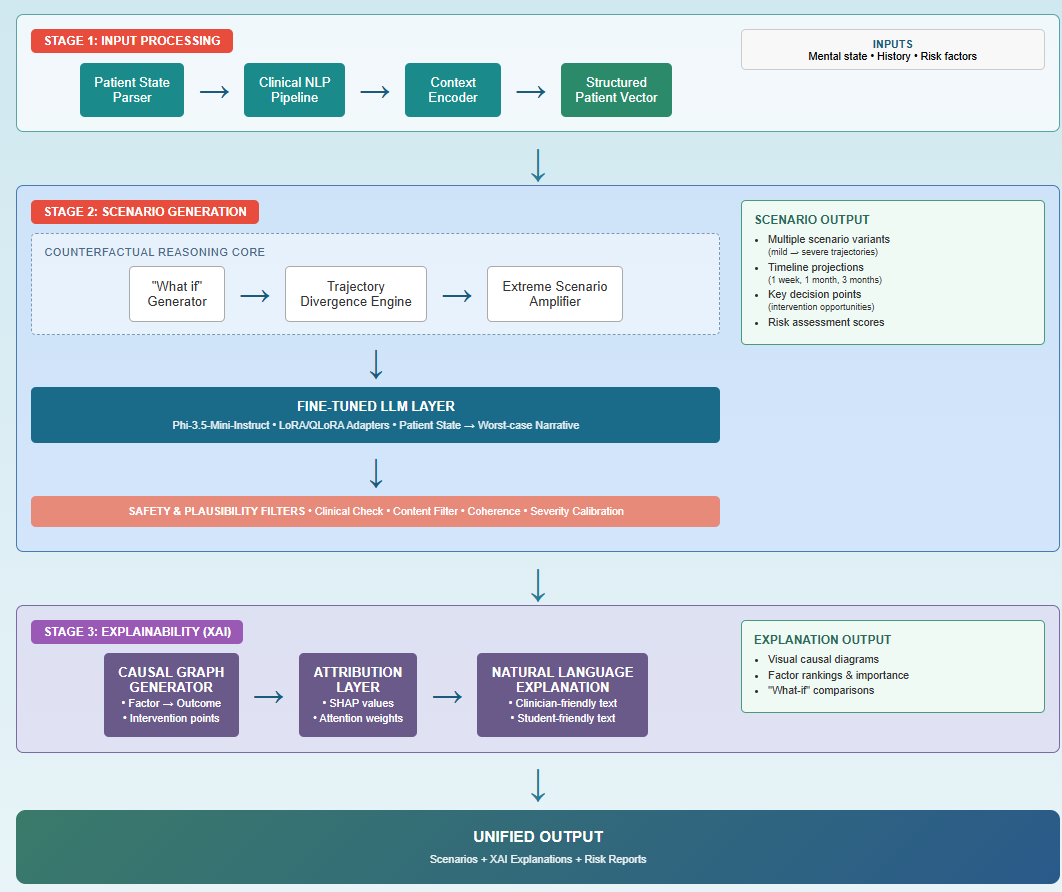
\includegraphics[width=\columnwidth]{images/Flow_diagram.png}
\caption{System architecture: seven-stage pipeline from clinical note to evidence-attributed crisis scenarios.}
\label{fig:architecture}
\end{figure}

Algorithm~\ref{alg:pipeline} presents the complete pipeline procedure. Given a clinical note $\mathcal{N}$, the pipeline produces structured clinical factors $\mathcal{S}$, scenario narratives $\mathcal{R}$, and evidence attribution mappings $\mathcal{E}$.

\begin{algorithm}[h]
\caption{Complete Pipeline Procedure}
\label{alg:pipeline}
\begin{algorithmic}[1]
\REQUIRE Clinical note $\mathcal{N}$, fine-tuned model $\mathcal{M}$
\ENSURE Factors $\mathcal{S}$, Scenarios $\mathcal{R}$, Attribution $\mathcal{E}$
\STATE \textbf{Stage 1:} $\mathcal{S}_{\text{raw}} \leftarrow \text{Extract}(\mathcal{M}, \mathcal{N})$
\STATE \textbf{Stage 2:} $\mathcal{S}_{\text{norm}} \leftarrow \text{Normalize}(\mathcal{S}_{\text{raw}}, \mathcal{N})$
\STATE \textbf{Stage 3:} $\mathcal{S} \leftarrow \text{Enrich}(\mathcal{S}_{\text{norm}}, \mathcal{N})$
\STATE \textbf{Stage 4:} $\mathcal{C} \leftarrow \text{DetectSignals}(\mathcal{N})$
\STATE \textbf{Stage 5:} $\mathcal{G} \leftarrow \text{GateBranches}(\mathcal{S}, \mathcal{C})$
\STATE \textbf{Stage 6:} $\mathcal{R} \leftarrow \emptyset$
\FOR{each branch $b \in \{A, B, C\}$}
    \IF{$\mathcal{G}[b] = \text{ACTIVE}$}
        \STATE $\mathcal{R}[b] \leftarrow \text{TreeOfThoughts}(b, \mathcal{S}, \mathcal{N})$
    \ELSE
        \STATE $\mathcal{R}[b] \leftarrow \text{``NOT APPLICABLE''}$
    \ENDIF
\ENDFOR
\STATE \textbf{Stage 7:} $\mathcal{E} \leftarrow \text{AttributeEvidence}(\mathcal{R}, \mathcal{N})$
\RETURN $(\mathcal{S}, \mathcal{R}, \mathcal{E})$
\end{algorithmic}
\end{algorithm}

\subsection{Stage 1: Clinical Factor Extraction}

The extraction stage employs a fine-tuned large language model to transform unstructured discharge summaries into structured JSON representations conforming to a DSM-5/ICD-11 grounded schema.

\textbf{Base Model.} We employ Microsoft Phi-3.5-Mini-Instruct (3.82B parameters), a decoder-only transformer architecture comprising 32 layers with 32 attention heads, hidden dimension $d_{\text{model}} = 3072$, and vocabulary size $|\mathcal{V}| = 32{,}064$. Although the model supports 128K token context, we constrain sequences to 2048 tokens for computational efficiency.

\textbf{LoRA Fine-Tuning.} Low-Rank Adaptation (LoRA) \cite{b19} enables parameter-efficient fine-tuning by freezing pre-trained weights $W_0$ and learning low-rank decomposition matrices. For weight matrix $W_0 \in \mathbb{R}^{d \times k}$, the adapted weight is:
\begin{equation}
    W = W_0 + \frac{\alpha}{r} BA
\end{equation}
where $B \in \mathbb{R}^{d \times r}$, $A \in \mathbb{R}^{r \times k}$, rank $r = 32$, and scaling factor $\alpha = 64$. We apply LoRA to all attention and feed-forward projections: $\{W_q, W_k, W_v, W_o, W_{\text{gate}}, W_{\text{up}}, W_{\text{down}}\}$, yielding 50.3M trainable parameters (1.30\% of total).

\textbf{Training Objective.} The model minimizes cross-entropy loss over target JSON sequences:
\begin{equation}
    \mathcal{L} = -\frac{1}{T} \sum_{t=1}^{T} \log P_\theta(y_t \mid y_{<t}, \mathcal{N})
\end{equation}
where $\mathcal{N}$ is the input note and $y = (y_1, \ldots, y_T)$ is the target JSON.

\textbf{Extraction Schema.} Table~\ref{tab:schema} defines the 14-field extraction schema. Each field has constrained value spaces ensuring structured, validated output.

\begin{table}[h]
\caption{Clinical Factor Extraction Schema}
\label{tab:schema}
\centering
\small
\begin{tabular}{@{}p{2.0cm}p{3.8cm}p{1.6cm}@{}}
\toprule
\textbf{Field} & \textbf{Description} & \textbf{Type} \\
\midrule
primary\_dx & Primary diagnosis & ICD-10 F01--99 \\
dsm5\_category & DSM-5 classification & Categorical \\
severity & Symptom severity & 4-level scale \\
suicide\_risk & Ideation, plan, attempt & Boolean$\times$3 \\
substance\_use & Alcohol, drugs, toxicology & Multi-field \\
medications & Current prescriptions & List \\
social\_support & Family, housing, employment & Multi-field \\
treatment\_history & Prior hospitalizations & Integer \\
\bottomrule
\end{tabular}
\end{table}

\subsection{Stage 2: Post-Extraction Normalization}

Raw extractions may contain inconsistencies requiring validation. This stage performs three normalization operations.

\textbf{ICD Code Validation.} Extracted ICD codes are validated against an authoritative lookup table $\mathcal{I}$ mapping codes to DSM-5 categories. Mismatched codes are corrected:
\begin{equation}
    c' = \begin{cases}
        \mathcal{I}(c)_{\text{corrected}} & \text{if mismatch detected} \\
        c & \text{otherwise}
    \end{cases}
\end{equation}

\textbf{Diagnosis Reconciliation.} The extracted primary diagnosis is cross-referenced against the ``Discharge Diagnosis'' section extracted via pattern matching, ensuring consistency with documented clinical conclusions.

\textbf{Redaction Resolution.} For privacy-redacted entities (e.g., ``[REDACTED] Disease''), contextual keyword co-occurrence infers the original diagnosis. For instance, presence of ``chorea'' and ``hereditary'' suggests Huntington's disease with high confidence.

\subsection{Stage 3: Context Enrichment}

The fixed extraction schema cannot capture all clinically relevant factors. The enrichment module scans the note for seven categories using pattern matching:
\begin{equation}
    \mathcal{E}_{\text{context}} = \bigcup_{c \in \mathcal{C}} \text{PatternMatch}(\mathcal{N}, \mathcal{P}_c)
\end{equation}
where $\mathcal{C}$ includes housing, caregiver, trauma, weight, functional, prognosis, and legal factors. Example patterns: \texttt{homeless}/\texttt{evict*}/\texttt{shelter} for housing; \texttt{sexual*abus*}/\texttt{PTSD} for trauma.

\subsection{Stage 4: Negation-Aware Critical Signal Detection}

Clinical notes frequently document both active concerns and explicitly denied symptoms. Distinguishing ``threatened to jump'' (active signal) from ``denies suicidal ideation'' (negated signal) is critical for accurate risk assessment.

Algorithm~\ref{alg:negation} formalizes the detection procedure. For each pattern match, a 40-character lookback window is examined for negation terms. Matches preceded by negators (``denies,'' ``no,'' ``negative for'') are classified as negated; others are flagged as active signals requiring immediate attention.

\begin{algorithm}[h]
\caption{Negation-Aware Signal Detection}
\label{alg:negation}
\begin{algorithmic}[1]
\REQUIRE Note $\mathcal{N}$, pattern sets $\mathcal{P} = \{\mathcal{P}_{\text{sui}}, \mathcal{P}_{\text{vio}}, \mathcal{P}_{\text{wpn}}\}$
\ENSURE Active signals $\mathcal{A}$, Negated signals $\mathcal{D}$
\STATE $\mathcal{A}, \mathcal{D} \leftarrow \emptyset, \emptyset$
\STATE $\mathcal{N}_L \leftarrow \text{lowercase}(\mathcal{N})$
\STATE $\text{NEG} \leftarrow \{\text{``denies''}, \text{``no ''}, \text{``not ''}, \text{``never''}, \text{``negative''}\}$
\FOR{each category $c \in \{\text{sui}, \text{vio}, \text{wpn}\}$}
    \FOR{each pattern $p \in \mathcal{P}_c$}
        \FOR{each match $m$ at position $i$ in $\mathcal{N}_L$}
            \STATE $\text{ctx} \leftarrow \mathcal{N}_L[\max(0, i-40) : i]$
            \IF{$\exists n \in \text{NEG} : n \in \text{ctx}$}
                \STATE $\mathcal{D} \leftarrow \mathcal{D} \cup \{(c, m, \text{``negated''})\}$
            \ELSE
                \STATE $\mathcal{A} \leftarrow \mathcal{A} \cup \{(c, m, \text{``active''})\}$
            \ENDIF
        \ENDFOR
    \ENDFOR
\ENDFOR
\RETURN $(\mathcal{A}, \mathcal{D})$
\end{algorithmic}
\end{algorithm}

Signal categories include suicide indicators (``kill myself,'' ``end my life,'' ``overdose''), violence indicators (``assault,'' ``homicidal''), and weapons access (``gun,'' ``firearm'').

\subsection{Stage 5: Evidence-Based Branch Gating}

To prevent hallucinated scenarios unsupported by clinical evidence, the framework implements conditional branch activation. Three scenario branches are defined:
\begin{itemize}
    \item \textbf{Branch A} (Psychiatric Deterioration): Always active
    \item \textbf{Branch B} (Substance Escalation): Conditional
    \item \textbf{Branch C} (Social/Environmental Collapse): Always active
\end{itemize}

Branch B activation requires evidence satisfying predicate $\phi_B$:
\begin{equation}
    \phi_B(\mathcal{S}) = (s_{\text{alcohol}} \neq \emptyset) \lor (s_{\text{drugs}} \neq \emptyset) \lor (s_{\text{tox}} = \text{positive})
\end{equation}
If $\neg \phi_B(\mathcal{S})$, Branch B outputs ``NOT APPLICABLE No substance use evidence,'' preventing fabricated substance abuse trajectories.

\subsection{Stage 6: Tree-of-Thoughts Scenario Generation}

For each active branch, structured counterfactual scenarios are generated through a three-step Tree-of-Thoughts (ToT) reasoning process. Algorithm~\ref{alg:tot} formalizes the procedure.

\begin{algorithm}[h]
\caption{Tree-of-Thoughts Scenario Generation}
\label{alg:tot}
\begin{algorithmic}[1]
\REQUIRE Branch $b$, factors $\mathcal{S}$, note excerpt $\mathcal{N}_e$, LLM $\mathcal{M}$
\ENSURE Scenario narrative $R_b$
\STATE \textcolor{gray}{\textit{// Step 1: Trigger Identification}}
\STATE $\text{prompt}_1 \leftarrow \text{BuildPrompt}(b, \mathcal{S}, \mathcal{N}_e, \text{``triggers''})$
\STATE $T_b \leftarrow \mathcal{M}(\text{prompt}_1)$ \COMMENT{3--5 triggers with evidence}
\IF{$|T_b| = 0$}
    \RETURN ``No triggering factors identified''
\ENDIF
\STATE \textcolor{gray}{\textit{// Step 2: Causal Chain Reasoning}}
\STATE $\text{prompt}_2 \leftarrow \text{BuildPrompt}(b, T_b, \mathcal{S}, \text{``causal''})$
\STATE $C_b \leftarrow \mathcal{M}(\text{prompt}_2)$ \COMMENT{4--6 escalation steps}
\STATE \textcolor{gray}{\textit{// Step 3: Scenario Narrative Synthesis}}
\STATE $\text{prompt}_3 \leftarrow \text{BuildPrompt}(b, T_b, C_b, \mathcal{S}, \mathcal{N}_e)$
\STATE $R_b \leftarrow \mathcal{M}(\text{prompt}_3)$
\RETURN $R_b$
\end{algorithmic}
\end{algorithm}

\textbf{Step 1: Trigger Identification.} The LLM identifies 3--5 triggering factors from the clinical note, each with direct evidence citations and mental health relevance ratings (scale 1--10).

\textbf{Step 2: Causal Chain Reasoning.} Given identified triggers, the LLM constructs 4--6 sequential escalation steps, each describing the mechanism linking the previous step to increased crisis risk.

\textbf{Step 3: Scenario Narrative Synthesis.} The final step synthesizes triggers and causal chains into a coherent crisis narrative, including: (a) detailed scenario description, (b) observable warning signs, (c) projected crisis endpoint, (d) clinical preparedness recommendations, and (e) plausibility rating.

\subsection{Stage 7: Evidence Attribution}

The final stage grounds generated scenarios in source text, providing post-hoc explainability. Algorithm~\ref{alg:attribution} formalizes the evidence attribution procedure.

\begin{algorithm}[h]
\caption{Evidence Attribution with Nexus Detection}
\label{alg:attribution}
\begin{algorithmic}[1]
\REQUIRE Scenarios $\mathcal{R}$, note $\mathcal{N}$, threshold $\tau = 0.45$
\ENSURE Attribution map $\mathcal{E}$, nexus factors $\mathcal{X}$
\STATE $\mathcal{E} \leftarrow \{\}$; $\mathcal{X} \leftarrow \emptyset$
\FOR{each branch $b \in \{A, B, C\}$}
    \STATE $Q_b \leftarrow \text{ExtractQuotes}(\mathcal{R}[b])$
    \FOR{each quote $q \in Q_b$}
        \STATE \textcolor{gray}{\textit{// Try exact match first}}
        \IF{$q_{\text{lower}} \in \mathcal{N}_{\text{lower}}$}
            \STATE $\mathcal{E}[b] \leftarrow \mathcal{E}[b] \cup \{(q, \text{span}, \text{``exact''})\}$
        \ELSE
            \STATE \textcolor{gray}{\textit{// Fall back to fuzzy match}}
            \STATE $s^* \leftarrow \arg\max_{s \in \text{Windows}(\mathcal{N})} \text{Sim}(q, s)$
            \IF{$\text{Sim}(q, s^*) \geq \tau$}
                \STATE $\mathcal{E}[b] \leftarrow \mathcal{E}[b] \cup \{(q, s^*, \text{``fuzzy''})\}$
            \ENDIF
        \ENDIF
    \ENDFOR
\ENDFOR
\STATE \textcolor{gray}{\textit{// Detect nexus factors}}
\FOR{each span $e$ across all $\mathcal{E}[b]$}
    \IF{$|\{b : e \in \mathcal{E}[b]\}| \geq 2$}
        \STATE $\mathcal{X} \leftarrow \mathcal{X} \cup \{e\}$
    \ENDIF
\ENDFOR
\RETURN $(\mathcal{E}, \mathcal{X})$
\end{algorithmic}
\end{algorithm}

\textbf{Span Location.} For each evidence quote $q$ extracted from generated scenarios, the algorithm first attempts exact substring matching (case-insensitive). If exact matching fails, fuzzy matching using the Ratcliff-Obershelp similarity metric is applied:
\begin{equation}
    \text{Sim}(q, s) = \frac{2 \cdot |\text{LCS}(q, s)|}{|q| + |s|}
\end{equation}
where LCS denotes the longest common subsequence. Spans with similarity $\geq 0.45$ are accepted.

\textbf{Nexus Factor Detection.} An evidence span supporting multiple branches constitutes a \textit{nexus factor} a single clinical element driving multiple crisis pathways. Nexus factors are assigned highest intervention priority, as addressing them may prevent multiple escalation trajectories simultaneously.

\textbf{Coverage Statistics.} Attribution coverage quantifies the proportion of the source note directly supporting generated scenarios:
\begin{equation}
    \text{Coverage} = \frac{\sum_{e \in \mathcal{E}} |e_{\text{end}} - e_{\text{start}}|}{|\mathcal{N}|}
\end{equation}

\section{Experimental Setup}

\subsection{Dataset: MIMIC-IV}

We use MIMIC-IV v3.1 \cite{b14}, filtering for mental health-related admissions:
\begin{equation}
    \mathcal{D} = \{(\mathcal{N}_i, \mathcal{S}_i)\} : \text{ICD}_i \in [\text{F01--F99}] \cup [290\text{--}319]
\end{equation}

\begin{table}[h]
\caption{Dataset Composition}
\label{tab:dataset}
\centering
\begin{tabular}{lrr}
\toprule
\textbf{Split} & \textbf{Patients} & \textbf{Examples} \\
\midrule
Training & 45,223 & 94,592 \\
Validation & 5,640 & 11,409 \\
Test & 5,640 & 11,916 \\
\midrule
\textbf{Total} & \textbf{56,503} & \textbf{117,917} \\
\bottomrule
\end{tabular}
\end{table}

\textbf{Label Distribution:} Severity levels (mild: 28.0\%, moderate: 24.6\%, severe: 34.9\%, critical: 12.5\%); DSM-5 categories (depressive: 31.9\%, anxiety: 20.0\%, substance: 19.5\%, neurocognitive: 14.0\%, other: 14.6\%).

\subsection{Training Configuration}

\begin{table}[h]
\caption{Hyperparameter Configuration}
\label{tab:hyperparams}
\centering
\begin{tabular}{ll}
\toprule
\textbf{Parameter} & \textbf{Value} \\
\midrule
Base model & Phi-3.5-Mini-Instruct (3.82B) \\
LoRA rank $r$ & 32 \\
LoRA alpha $\alpha$ & 64 \\
LoRA dropout & 0.05 \\
Learning rate & $2 \times 10^{-4}$ \\
Batch size (effective) & 64 \\
Gradient accumulation & 8 steps \\
Epochs & 5 \\
Warmup ratio & 0.03 \\
Max sequence length & 2048 tokens \\
Precision & FP16 \\
Optimizer & AdamW ($\beta_1=0.9, \beta_2=0.999$) \\
\midrule
Hardware & 4$\times$ Tesla V100-SXM2-32GB \\
Distributed & PyTorch DDP \\
\bottomrule
\end{tabular}
\end{table}

\section{Results and Analysis}

This section presents the experimental results in three parts: (1) training performance of the extraction model, (2) iterative pipeline development from baseline to final system, and (3) qualitative evaluation demonstrating system capabilities.

\subsection{Model Training Results}

The LoRA fine-tuned Phi-3.5-Mini-Instruct model was trained on 94,592 MIMIC-IV discharge summaries over 5 epochs (7,390 steps). Fig.~\ref{fig:training_curves} shows the training dynamics.

\begin{figure}[h]
\centering
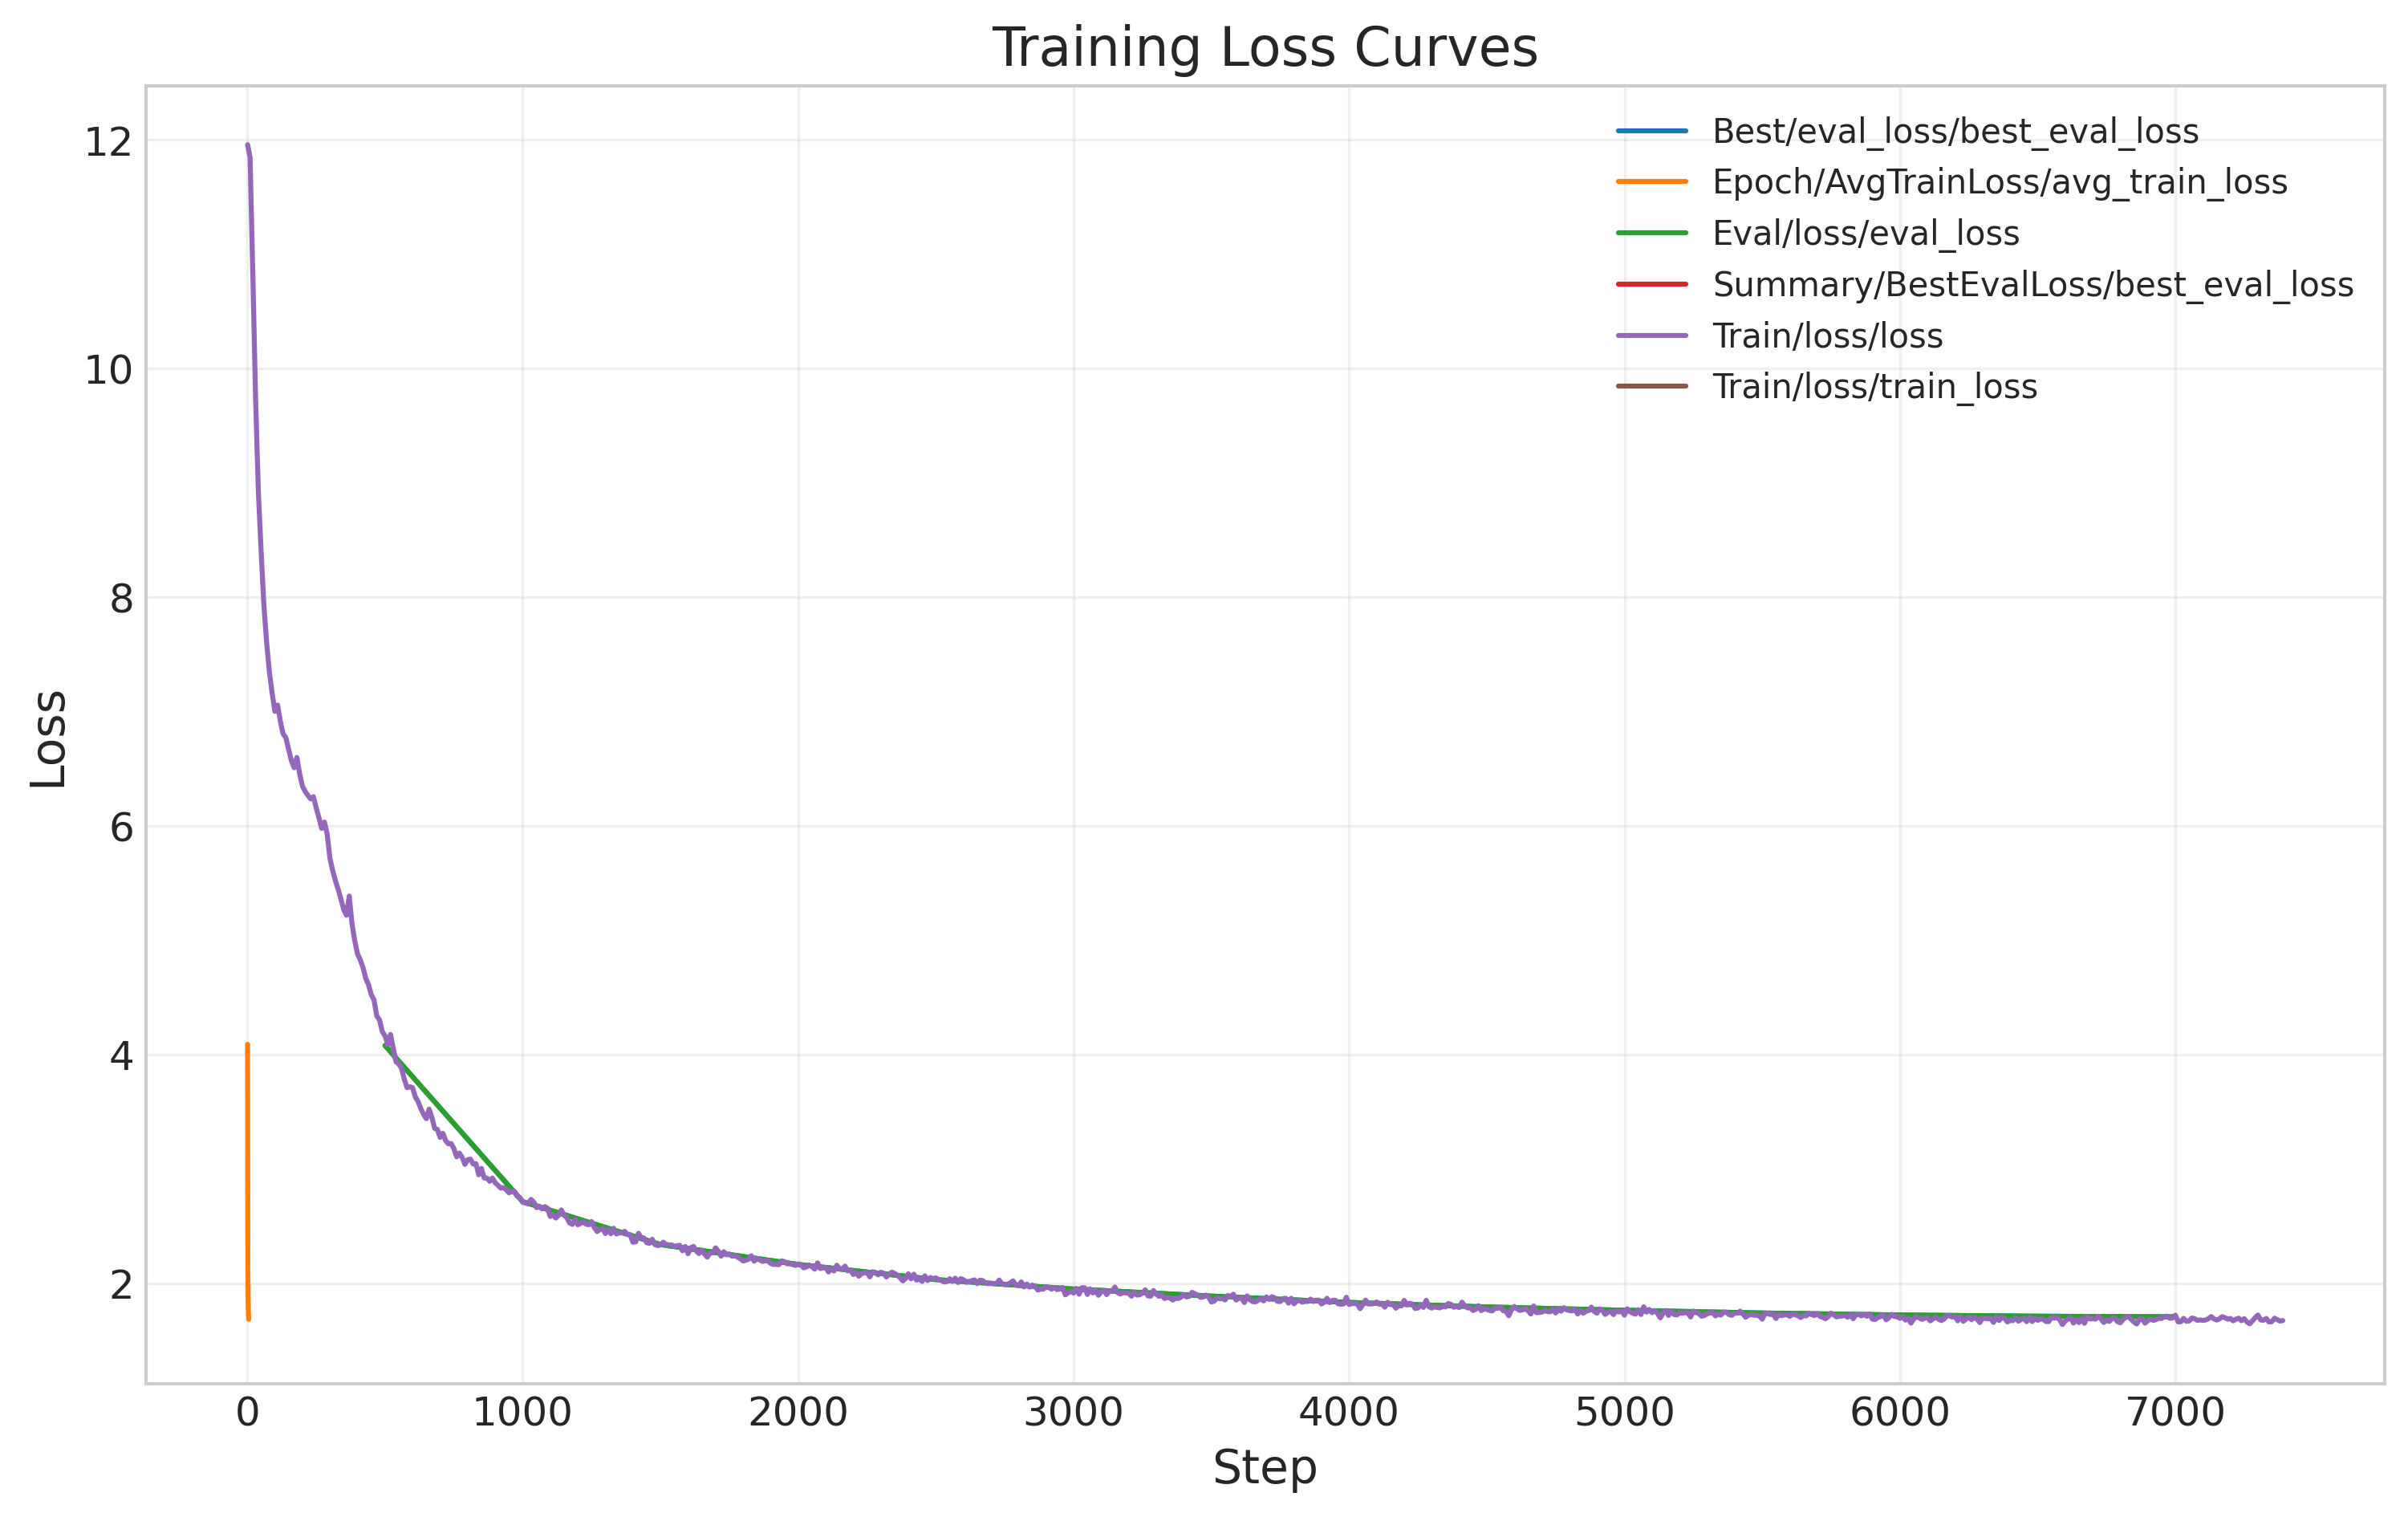
\includegraphics[width=\columnwidth]{images/combined_loss.png}
\caption{Training and evaluation loss curves. Evaluation loss decreases from 4.08 to 1.706 (58.2\% reduction) with no overfitting observed.}
\label{fig:training_curves}
\end{figure}

Table~\ref{tab:training_summary} summarizes the final training metrics. The model achieves 67.5\% token-level accuracy, indicating reliable JSON schema generation. Perplexity of 5.51 suggests the model confidently predicts structured output tokens.

\begin{table}[h]
\caption{Training Results Summary}
\label{tab:training_summary}
\centering
\begin{tabular}{@{}ll@{}}
\toprule
\textbf{Metric} & \textbf{Value} \\
\midrule
Training time & 35.8 hours \\
Total steps & 7,390 \\
Best evaluation loss & 1.706 \\
Final token accuracy & 67.5\% \\
Final perplexity & 5.51 \\
Trainable parameters & 50.3M (1.30\%) \\
Hardware & 4$\times$ V100-32GB \\
Throughput & 3.67 samples/sec \\
Total FLOPs & $1.096 \times 10^{19}$ \\
\bottomrule
\end{tabular}
\end{table}

Table~\ref{tab:checkpoints} shows the evaluation metrics at each 500-step checkpoint. The model exhibits rapid early learning, achieving 55.7\% token accuracy within the first 1,000 steps, followed by gradual refinement.

\begin{table}[h]
\caption{Training Progression at Evaluation Checkpoints}
\label{tab:checkpoints}
\centering
\small
\begin{tabular}{@{}rrrr@{}}
\toprule
\textbf{Step} & \textbf{Eval Loss} & \textbf{Token Acc.} & \textbf{Perplexity} \\
\midrule
500 & 4.079 & 41.6\% & 59.1 \\
1,000 & 2.713 & 55.7\% & 15.1 \\
2,000 & 2.164 & 61.8\% & 8.7 \\
3,000 & 1.949 & 64.3\% & 7.0 \\
4,000 & 1.832 & 65.8\% & 6.2 \\
5,000 & 1.764 & 66.6\% & 5.8 \\
6,000 & 1.722 & 67.2\% & 5.6 \\
7,000 & \textbf{1.706} & \textbf{67.5\%} & \textbf{5.5} \\
\bottomrule
\end{tabular}
\end{table}

Training exhibited stable gradient norms throughout, with a brief initial spike to 2.97 at step 20 that quickly stabilized to the 0.1--0.7 range for the remainder of training. The 3\% warmup schedule (222 steps) prevented sustained instability. GPU memory utilization remained under 11 GB per device (8.47 GB allocated, 10.13 GB peak), demonstrating that LoRA enables efficient fine-tuning on commodity hardware.

Fig.~\ref{fig:token_accuracy} illustrates the token accuracy progression. Accuracy increases rapidly during the first epoch (steps 0--1,478), achieving 55.7\% by step 1,000. Subsequent epochs show diminishing returns, with accuracy improving from 61.8\% (step 2,000) to 67.5\% (step 7,000) a pattern consistent with the model mastering structural JSON syntax early and refining semantic content extraction in later epochs.

\begin{figure}[h]
\centering
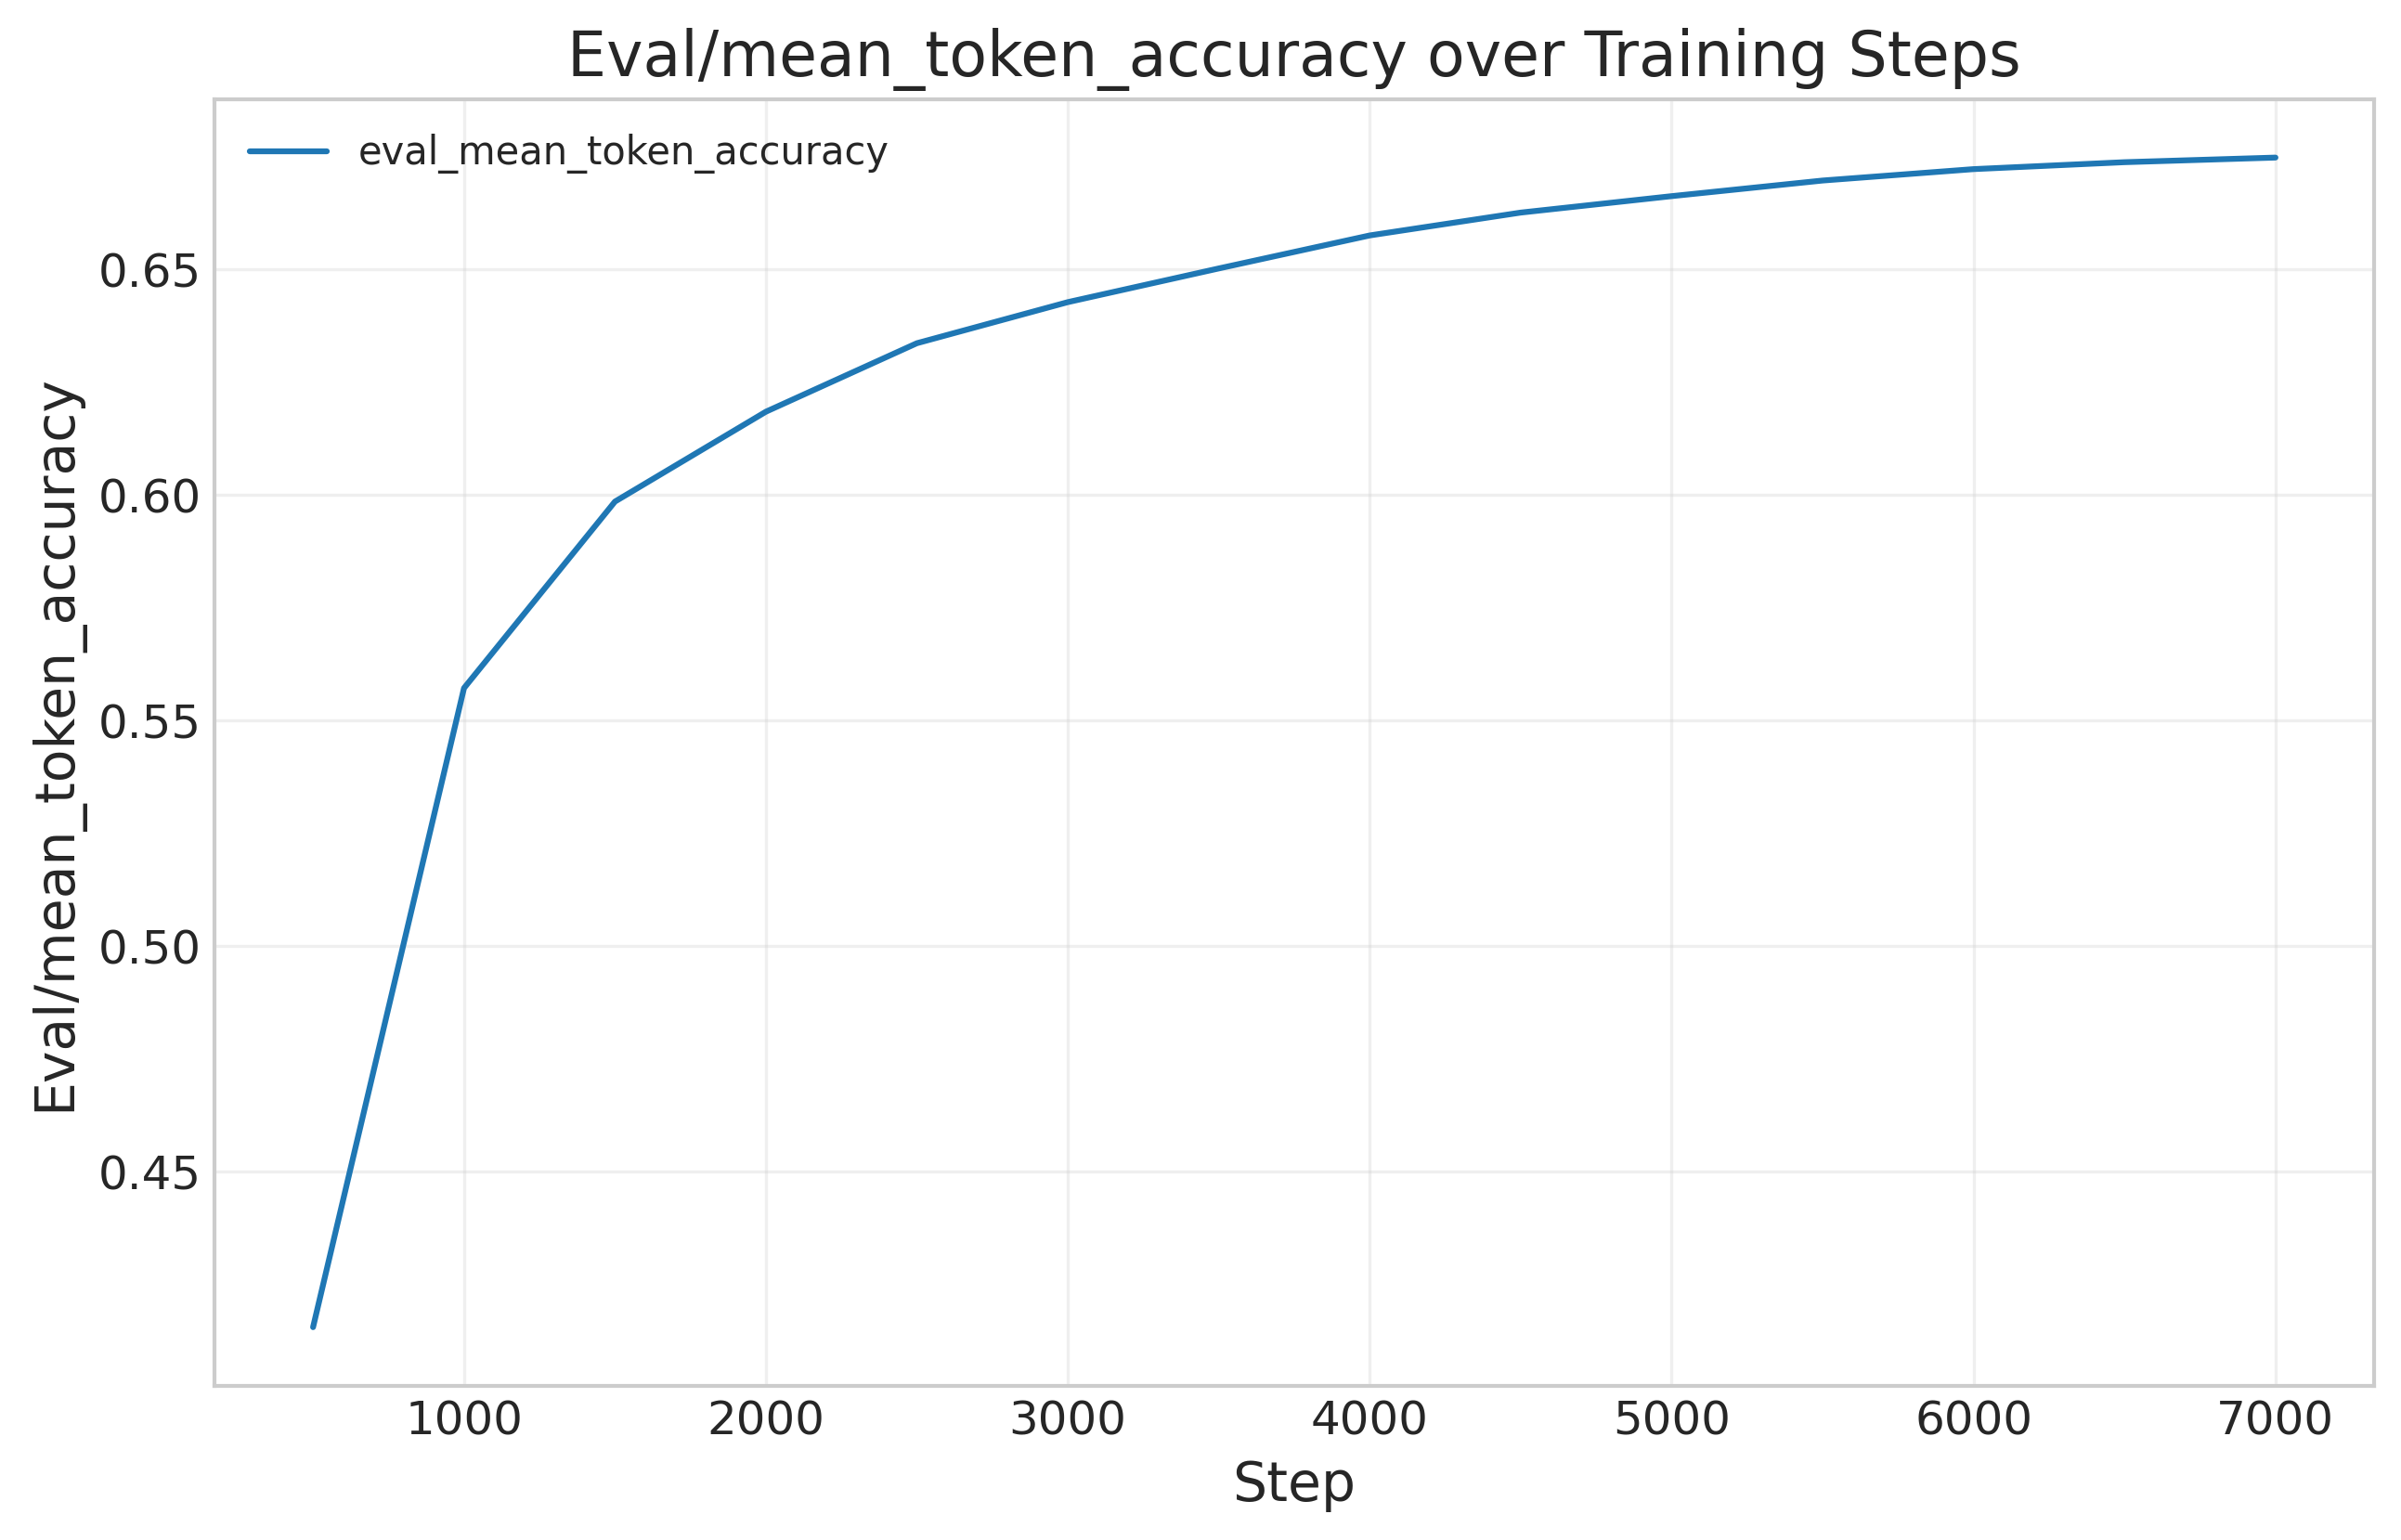
\includegraphics[width=\columnwidth]{images/Eval_mean_token_accuracy.png}
\caption{Token-level accuracy progression over 7,390 training steps. Rapid improvement in epoch 1 followed by gradual refinement. Final accuracy of 67.5\% indicates reliable JSON schema generation.}
\label{fig:token_accuracy}
\end{figure}

Fig.~\ref{fig:perplexity} shows the perplexity trajectory. Perplexity measures prediction uncertainty lower values indicate the model assigns higher probability to correct tokens. Initial perplexity of 59.1 (step 500) indicates the model was essentially guessing among 59 equally likely tokens. Final perplexity of 5.51 represents a 90.7\% reduction, meaning the model confidently narrows predictions to approximately 5--6 candidate tokens on average.

\begin{figure}[h]
\centering
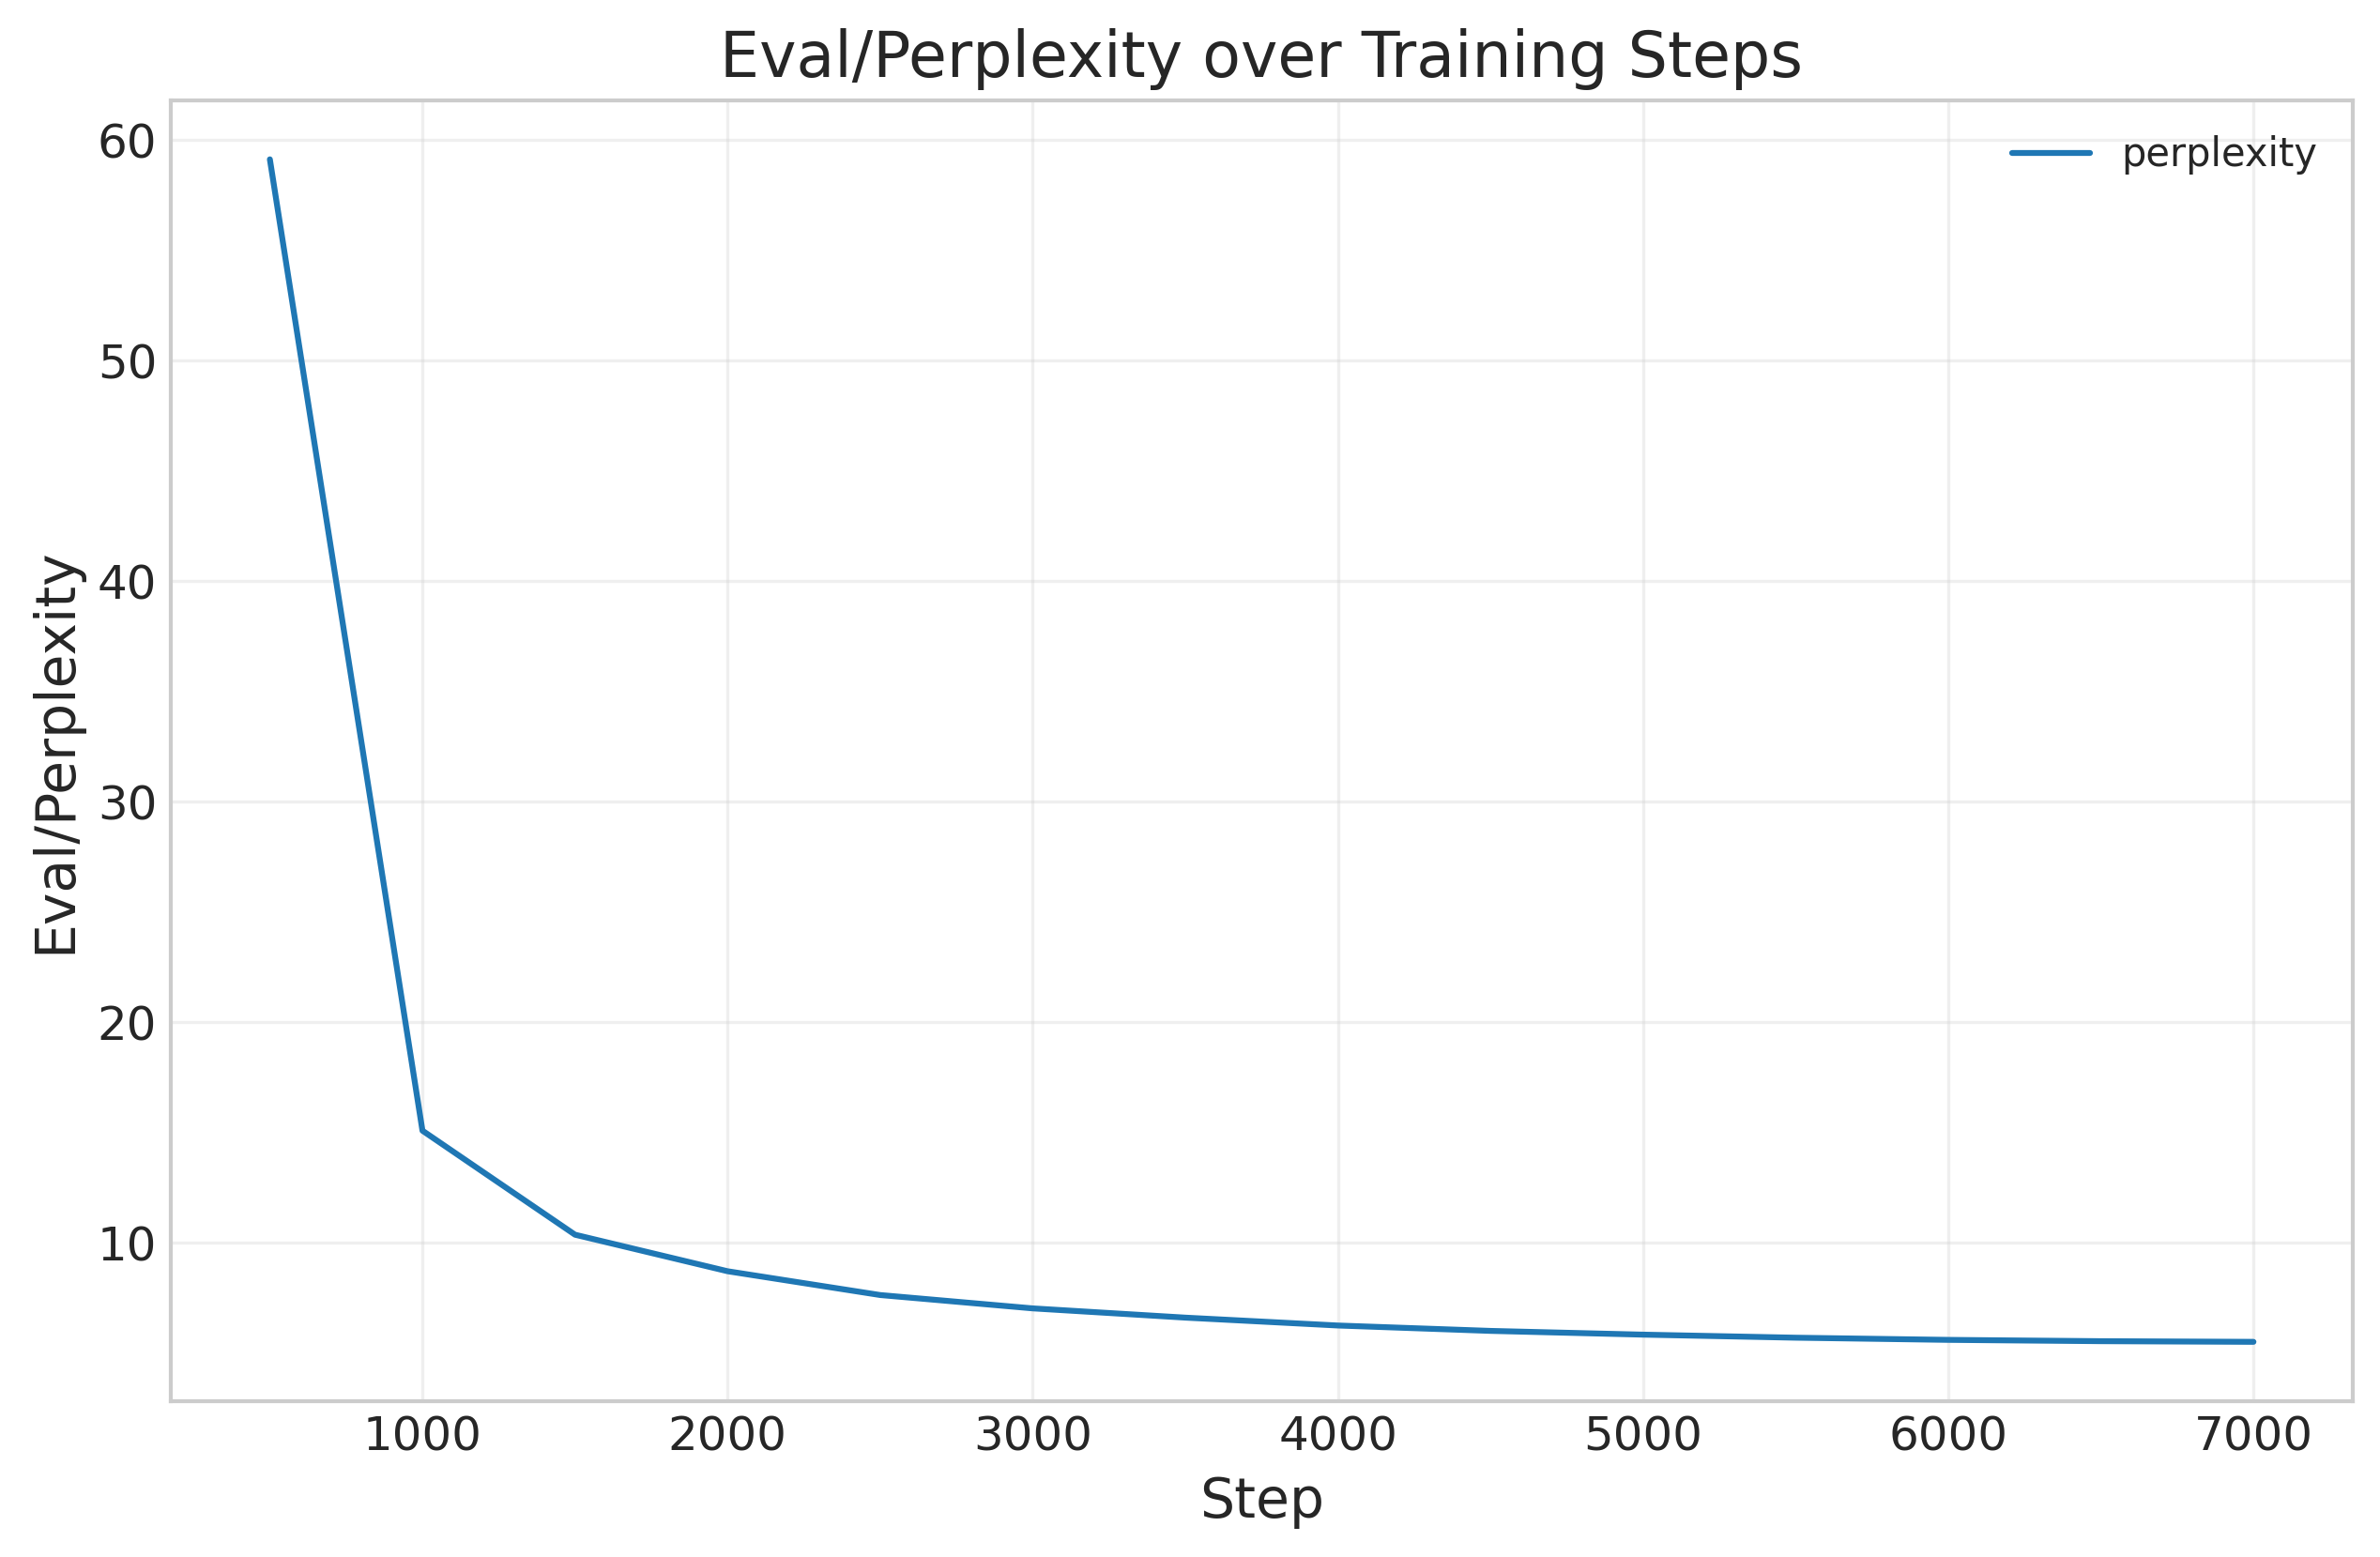
\includegraphics[width=\columnwidth]{images/Eval_Perplexity.png}
\caption{Evaluation perplexity over training. Perplexity decreases from 59.1 to 5.51 (90.7\% reduction), indicating significantly improved prediction confidence for structured output generation.}
\label{fig:perplexity}
\end{figure}

\subsection{Pipeline Evolution and Ablation Analysis}

The framework underwent iterative development through four versions, each addressing limitations identified in the previous iteration. Table~\ref{tab:evolution} summarizes the progression from baseline to final system.

\begin{table}[h]
\caption{Pipeline Version Evolution}
\label{tab:evolution}
\centering
\small
\begin{tabular}{@{}p{0.6cm}p{3.4cm}p{3.2cm}@{}}
\toprule
\textbf{Ver.} & \textbf{Capabilities Added} & \textbf{Problems Addressed} \\
\midrule
V1 & Extract $\rightarrow$ Scenarios $\rightarrow$ Report & Baseline 3-phase pipeline \\
\midrule
V2 & +ICD normalization, +Critical signal scanner, +Branch gating, +Consistency checks & Extraction errors, missed safety signals, irrelevant scenarios \\
\midrule
V3 & +Context enrichment, +Negation awareness, +Deduplication & Missing social context, false positive alerts \\
\midrule
V4 & +Evidence attribution, +Nexus detection, +DOCX export & Lack of explainability, no traceability \\
\bottomrule
\end{tabular}
\end{table}

\subsubsection{V1 Baseline: Three-Phase Pipeline}

The initial system implemented a straightforward three-phase architecture: (1) clinical factor extraction via the fine-tuned model, (2) Tree-of-Thoughts scenario generation across three branches, and (3) clinical report synthesis. While functional, V1 exhibited several critical limitations:

\textbf{Problem 1: No validation layer.} Extraction errors propagated directly to scenario generation. ICD code misclassifications and incorrect severity assignments persisted in final outputs.

\textbf{Problem 2: Unconditional branch execution.} All three scenario branches (psychiatric, substance, social) executed regardless of clinical relevance. Patients with no documented substance use received fabricated substance abuse trajectories.

\textbf{Problem 3: No safety signal detection.} The system relied entirely on the LLM to identify critical signals. If the model failed to extract suicide or violence indicators, they were missed completely.

\textbf{Problem 4: Schema rigidity.} The fixed 14-field extraction schema missed contextually important factors such as housing instability, caregiver loss, and trauma history.

\subsubsection{V2 Enhanced: Validation and Safety Pipeline}

Version 2 introduced four new modules addressing V1's validation and safety gaps:

\textbf{Stage 1.5 (Normalization):} Validates extracted ICD codes against an authoritative lookup table, reconciles primary diagnosis with the ``Discharge Diagnosis'' section, and classifies diseases into DSM-5 categories. This caught and corrected diagnostic errors before downstream processing.

\textbf{Stage 1.6 (Critical Signal Detection):} Implements rule-based regex scanning for suicide, violence, and weapons-related signals. This model-independent safety layer ensures critical signals are never missed, regardless of extraction model performance.

\textbf{Stage 1.7 (Branch Gating):} Evaluates clinical evidence before activating each scenario branch. Branch B (Substance Escalation) requires documented alcohol use, drug use, or positive toxicology. Patients lacking such evidence receive ``NOT APPLICABLE'' rather than hallucinated substance scenarios.

\textbf{Stage 3.5 (Consistency Checker):} Performs final validation including risk tier override when critical signals are detected, resolution of ``unknown'' severity values, and acknowledgment of gated branches in the final report.

\subsubsection{V3 Refined: Context and Precision Pipeline}

Version 3 addressed remaining gaps in contextual understanding and alert precision:

\textbf{Stage 1.55 (Context Enrichment):} Scans the clinical note for seven contextual categories not captured by the extraction schema: housing crisis, caregiver loss, trauma history, weight change, functional decline, clinician prognosis, and legal status. These enriched factors are injected into the structured representation for downstream scenario generation.

\textbf{Negation-Aware Signal Detection:} The critical signal scanner was enhanced with a 40-character lookback window to detect negation terms. The statement ``Self-injury: denies'' is now correctly classified as negated, while ``threatened to jump out her window'' triggers an active alert. This eliminated false positive alerts that plagued V2.

\textbf{Alert Deduplication:} Multiple matches of the same signal pattern are consolidated before output, reducing redundant alerts.

Table~\ref{tab:version_comparison} summarizes the observed error patterns across versions based on qualitative review of pipeline outputs during development.

\begin{table}[h]
\caption{Observed Error Patterns Across Pipeline Versions}
\label{tab:version_comparison}
\centering
\begin{tabular}{@{}lrrr@{}}
\toprule
\textbf{Error Type} & \textbf{V1} & \textbf{V2} & \textbf{V3} \\
\midrule
ICD code misclassification & Frequent & Rare & Rare \\
Missed critical signals & Frequent & None & None \\
Irrelevant substance scenarios & Frequent & None & None \\
False positive alerts & -- & Frequent & None \\
Missing housing/trauma context & Frequent & Frequent & Rare \\
\bottomrule
\end{tabular}
\end{table}

\subsubsection{V4 Final: Explainable Attribution}

While V3 produced clinically appropriate scenarios, it lacked explainability clinicians could not verify which portions of the original note supported each generated claim. Version 4 addresses this through:

\textbf{Stage 4 (Evidence Attribution):} Maps every scenario trigger and risk factor back to specific character spans in the source clinical note. The algorithm first attempts exact substring matching; if unsuccessful, fuzzy matching via Ratcliff-Obershelp similarity ($\tau \geq 0.45$) locates paraphrased evidence.

\textbf{Nexus Factor Detection:} Identifies evidence spans supporting multiple branches simultaneously. A ``housing crisis'' mention supporting both psychiatric deterioration (Branch A) and social collapse (Branch C) is flagged as a nexus factor with elevated intervention priority.

\textbf{Coverage Statistics:} Computes the proportion of the source note directly grounding generated scenarios. Higher coverage indicates stronger evidence basis; low coverage flags potentially speculative outputs.

\subsection{Illustrative Input-Output Example}

Before presenting the full qualitative case study, we include actual excerpts from a processed clinical note to demonstrate how the framework transforms raw documentation into structured preparedness output. Table~\ref{tab:mini_example} shows verbatim input text and corresponding system outputs.

\begin{table}[h]
\caption{Actual Input-Output Example from Pipeline}
\label{tab:mini_example}
\centering
\small
\begin{tabular}{@{}p{3.2cm}p{4.4cm}@{}}
\toprule
\textbf{Input Note (Verbatim)} & \textbf{System Output} \\
\midrule
``Her apt has been auctioned off and will be homeless at the end of the week.'' & \texttt{[ENRICH] Housing crisis detected: homelessness, imminent homelessness, housing loss. Updated housing\_status to `homeless'.} Branch C activated. \\
\midrule
``She threatened to jump out her 10 story window if the took her to one of her outpatient treators.'' & \texttt{CRITICAL SAFETY ALERT: SUICIDE/SELF-HARM SIGNAL: `jump out'.} Risk tier override: HIGH. \\
\midrule
``Self-injury: denies'' / ``Access to weapons: denies'' & \texttt{[NEGATED] violence: `weapons'}   correctly classified as negated and excluded from active alerting. \\
\midrule
Toxicology: ``Ethanol-NEG, opiates-NEG, cocaine-NEG, amphetm-NEG'' & \texttt{Branch B: NOT APPLICABLE   No substance use evidence. Data: alcohol=none, drugs=none, tox\_screen=negative.} \\
\midrule
``wide-based and ataxic'' / ``monosyllabic phrases'' / ``difficulty caring for self'' & \texttt{[ENRICH] Functional decline detected: self-care difficulty, ataxic gait, monosyllabic speech, speech latency. Homebound duration: a year.} \\
\bottomrule
\end{tabular}
\end{table}

This example illustrates that the framework performs evidence-grounded transformations: housing language triggers enrichment and Branch C activation, explicit threats generate critical alerts with risk elevation, negated statements are correctly suppressed, negative toxicology gates out the substance pathway, and functional indicators are aggregated into enrichment factors supporting scenario plausibility. The input and output presented above are drawn from MIMIC-IV discharge summary (subject\_id: 11399055, hadm\_id: 25710274).

\subsection{Qualitative Case Study}

We demonstrate the complete V4 pipeline on a representative case drawn from the MIMIC-IV test set (subject\_id: 11399055, hadm\_id: 25710274):

\textbf{Patient Profile:} Female with Huntington's disease presenting with agitation following apartment auction notice. Note length: 4,832 characters.

\textbf{Stage 1 (Extraction):} The fine-tuned model extracts primary diagnosis (F02.80, Huntington's disease with behavioral disturbance), severity (severe), and medication history. Suicide risk fields: ideation=true, plan=false, attempt=false.

\textbf{Stage 2 (Normalization):} ICD code F02.80 validated against lookup table. Disease name originally redacted as ``[REDACTED] Disease'' is resolved to ``Huntington's'' via keyword co-occurrence (``chorea,'' ``hereditary,'' ``CAG repeat'').

\textbf{Stage 3 (Enrichment):} Seven enrichment categories evaluated:
\begin{itemize}
    \item Housing crisis: \textsc{detected} (``apartment auctioned,'' ``will be homeless'')
    \item Functional decline: \textsc{detected} (``ataxic gait,'' ``monosyllabic speech'')
    \item Trauma history: \textsc{detected} (``sexually molested in childhood'')
    \item Caregiver loss: \textsc{detected} (``daughter refusing contact'')
    \item Prognosis: \textsc{detected} (``progressive neurodegenerative'')
\end{itemize}

\textbf{Stage 4 (Critical Signals):}
\begin{itemize}
    \item \textsc{active}: ``threatened to jump out her 10 story window''
    \item \textsc{negated}: ``Self-injury: denies'' (correctly downgraded)
    \item \textsc{negated}: ``Access to weapons: denies'' (correctly downgraded)
\end{itemize}

\textbf{Stage 5 (Branch Gating):}
\begin{itemize}
    \item Branch A (Psychiatric): \textsc{active}
    \item Branch B (Substance): \textsc{gated}   no alcohol, drugs, or positive toxicology
    \item Branch C (Social): \textsc{active}
\end{itemize}

\textbf{Stage 6 (Scenario Generation):} Tree-of-Thoughts reasoning produces two scenarios. Branch A projects rapid cognitive decline with suicide risk escalation triggered by housing loss and family abandonment. Branch C projects complete social system collapse with homelessness and loss of psychiatric follow-up.

\textbf{Stage 7 (Evidence Attribution):}
\begin{itemize}
    \item Total evidence spans located: 11
    \item Exact matches: 8 (72.7\%)
    \item Fuzzy matches: 3 (27.3\%)
    \item Nexus factors: 2 (``homelessness,'' ``daughter refusing contact'')
    \item Note coverage: 14.2\%
\end{itemize}

The two nexus factors housing crisis and family estrangement support both Branch A and Branch C scenarios, indicating that intervention addressing these factors could mitigate multiple crisis pathways simultaneously.

% \subsection{Computational Performance}

% Table~\ref{tab:inference_perf} reports inference performance on a single NVIDIA A100-80GB GPU.

% \begin{table}[h]
% \caption{Inference Performance (Single A100-80GB)}
% \label{tab:inference_perf}
% \centering
% \begin{tabular}{@{}lr@{}}
% \toprule
% \textbf{Pipeline Stage} & \textbf{Time (s)} \\
% \midrule
% Stage 1: Extraction & 8.2 \\
% Stages 2--5: Normalization through Gating & 0.3 \\
% Stage 6: ToT Scenario Generation (2 branches) & 24.6 \\
% Stage 7: Evidence Attribution & 1.1 \\
% \midrule
% \textbf{Total Pipeline} & \textbf{34.2} \\
% \bottomrule
% \end{tabular}
% \end{table}

% The scenario generation stage dominates runtime due to three sequential LLM calls per active branch. Attribution adds minimal overhead (1.1s) despite iterating over all evidence spans.

\section{Discussion}

The results support two central claims of this work. First, structured clinical factor extraction can be learned reliably with parameter-efficient adaptation: the model converged to an evaluation loss of 1.706, token accuracy of 67.5\%, and perplexity of 5.51 while training only 1.30\% of total model parameters. Second, reliable clinical scenario generation requires more than extraction alone. The progression from V1 to V4 shows that post-extraction normalization, context enrichment, safety-aware filtering, branch gating, and evidence attribution are not peripheral additions; they are necessary components for converting raw LLM outputs into clinically interpretable preparedness scenarios.

\subsection{Interpretation of Findings}

The training curves indicate that the model learns output structure early and refines semantic fidelity later. Token accuracy improved rapidly in the first phase of training, suggesting that the model quickly internalized the JSON schema and general extraction format. The subsequent slower but consistent decrease in evaluation loss and perplexity indicates gradual improvement in the correctness of clinically meaningful field values rather than mere formatting. This distinction is important because structurally valid output alone is insufficient in a clinical pipeline; downstream stages depend on semantically correct diagnoses, severity labels, and risk indicators.

The version-wise pipeline analysis provides an equally important result: the best-performing system was not achieved by scaling the base model alone, but by progressively constraining and validating model behavior. V2 reduced missed critical signals and irrelevant branch execution by introducing normalization, explicit signal detection, and branch gating. V3 further improved practical reliability by incorporating context enrichment and negation awareness, thereby reducing false positive alerts and recovering clinically salient social factors omitted by the fixed extraction schema. V4 extended the system from clinically plausible generation to explainable generation by mapping generated claims back to source evidence spans. Taken together, these findings suggest that in high-stakes clinical NLP, architectural safeguards and post-hoc verification contribute as much to system trustworthiness as the underlying generative model.

\subsection{Clinical and Methodological Implications}

From a clinical perspective, the framework reframes mental health AI from retrospective risk classification to prospective preparedness support. Rather than outputting a scalar risk score, the system identifies plausible deterioration pathways, the clinical and social triggers associated with those pathways, and the source-note evidence supporting them. This is a more actionable representation for discharge planning, psychiatric triage, and crisis prevention because it supports intervention planning around concrete factors such as housing instability, family estrangement, or active suicidality.

The case study illustrates this shift clearly. The framework did not simply identify a high-risk patient; it separated psychiatric and social deterioration pathways, gated out the unsupported substance pathway, and identified nexus factors shared across active branches. Such outputs are more aligned with how clinicians reason about worsening trajectories in practice, where overlapping biological, psychiatric, and environmental stressors shape escalation.

Methodologically, the study also highlights a practical design principle for domain-specific LLM systems: deterministic modules remain valuable even when a strong generative model is available. Rule-based negation detection, branch gating, ICD reconciliation, and evidence matching each address failure modes that generative models alone do not resolve consistently. The resulting hybrid architecture is therefore not a workaround, but an intentional design choice for improving safety, controllability, and interpretability.

\subsection{Future Work}

Several directions follow naturally from these findings. The most immediate next step is rigorous expert evaluation using manually annotated corpora for structured extraction, branch activation correctness, and evidence attribution quality. Such evaluation would enable quantitative comparison against alternative clinical NLP baselines and would make it possible to assess whether the apparent qualitative gains of V3 and V4 translate into measurable reliability improvements.

Beyond annotation, clinician-in-the-loop studies are needed to test whether generated scenarios are useful in real decision workflows. In particular, future studies should examine whether scenario narratives, nexus factor identification, and evidence-grounded explanations improve preparedness planning, discharge decisions, or early intervention prioritization relative to conventional risk summaries.

At the modeling level, longitudinal extensions represent a promising direction. Incorporating multiple encounters, medication timelines, prior admissions, and evolving risk markers could support trajectory-aware counterfactual simulation rather than note-level scenario generation. Similarly, evidence attribution could be strengthened by combining text matching with learned alignment methods, retrieval-based grounding, or attention-informed attribution to better capture paraphrastic support.

Finally, broader validation across psychiatric, emergency, and community mental health datasets will be necessary to assess robustness, fairness, and portability. Such work is essential before deployment-oriented claims can be made.

\section{Conclusion}

This paper addressed a central limitation of existing mental health AI systems: although prior approaches can classify risk, they do not explain how deterioration may unfold or which documented factors support that trajectory. To address this gap, we proposed a seven-stage framework for counterfactual simulation of extreme mental health scenarios from clinical notes. The framework combines LoRA-based clinical factor extraction, post-extraction normalization, context enrichment, negation-aware critical signal detection, evidence-based branch gating, Tree-of-Thoughts scenario generation, and post-hoc evidence attribution.

The experimental results show that the extraction component can be learned effectively with parameter-efficient fine-tuning, achieving an evaluation loss of 1.706, token-level accuracy of 67.5\%, and perplexity of 5.51 on 94,592 MIMIC-IV discharge summaries. More importantly, the version-wise evolution from V1 to V4 demonstrates that reliable clinical scenario generation depends on architectural safeguards beyond the base LLM. Normalization reduced extraction inconsistencies, negation-aware signal detection improved safety, branch gating prevented unsupported scenario generation, and evidence attribution made the final outputs traceable to source documentation.

The resulting system moves beyond black-box prediction toward evidence-grounded clinical preparedness support. Instead of producing only a risk score, it identifies plausible crisis pathways, highlights shared nexus factors across pathways, and links generated claims back to supporting text spans in the note. This makes the framework more aligned with clinical reasoning and more suitable for use in discharge planning, psychiatric triage, and early intervention workflows.

Overall, this work contributes an end-to-end and explainable pipeline for mental health crisis preparedness that integrates structured extraction, safety-aware validation, constrained generation, and traceable attribution within a single framework. While further clinician evaluation and external validation are necessary before deployment, the present results establish a strong methodological foundation for evidence-grounded counterfactual reasoning in clinical mental health applications.

\section*{Acknowledgment}

The authors acknowledge the MIT Laboratory for Computational Physiology and PhysioNet for providing access to the MIMIC-IV clinical database used in this study.

\begin{thebibliography}{00}

\bibitem{b1} GBD 2019 Mental Disorders Collaborators, ``Global burden of 12 mental disorders in 204 countries,'' \textit{Lancet Psychiatry}, vol. 9, no. 2, pp. 137--150, 2022.

\bibitem{b2} B. G. Teferra et al., ``NLP for mental health interventions: Systematic review,'' \textit{Transl. Psychiatry}, vol. 13, p. 309, 2023.

\bibitem{b3} E. Sezgin et al., ``Extracting medical information from free-text,'' \textit{JMIR Form. Res.}, vol. 7, e43014, 2023.

\bibitem{b4} X. Xu et al., ``Mental-LLM: LLMs for mental health prediction,'' \textit{Proc. ACM IMWUT}, vol. 8, no. 1, pp. 1--32, 2024.

\bibitem{b5} Z. Guo et al., ``LLMs for mental health applications: Systematic review,'' \textit{JMIR Mental Health}, vol. 11, e57400, 2024.

\bibitem{b6} Y. Hua et al., ``LLMs in mental health care: Scoping review,'' \textit{arXiv:2401.02984}, 2024.

\bibitem{b7} A. M. Alkalbani et al., ``LLMs in medical specialties: Systematic review,'' \textit{Information}, vol. 16, no. 6, p. 489, 2025.

\bibitem{b8} M. Prosperi et al., ``Clinical potential of counterfactual AI,'' \textit{The Lancet}, vol. 403, pp. 1063--1065, 2024.

\bibitem{b9} I. Gat et al., ``Counterfactual modeling with fine-tuned LLMs,'' \textit{arXiv:2601.14590}, 2026.

\bibitem{b10} J. Amann et al., ``Explainability for AI in healthcare: Systematic review,'' \textit{BMC Med. Inform. Decis. Mak.}, vol. 20, p. 310, 2020.

\bibitem{b11} S. M. Lundberg and S.-I. Lee, ``From explainability to action: Generative XAI framework,'' \textit{arXiv:2510.13828}, 2025.

\bibitem{b14} A. Johnson et al., ``MIMIC-IV, a freely accessible EHR dataset,'' \textit{Sci. Data}, vol. 10, p. 1, 2023.

\bibitem{b16} S. K. Lho et al., ``LLMs for detecting depression and suicide,'' \textit{JAMA Netw. Open}, vol. 8, no. 5, e2511922, 2025.

\bibitem{b17} W. Kim and C. Wang, ``LLMs for interpretable mental health diagnosis with DSM-5,'' \textit{LLM4Health Workshop}, 2025.

\bibitem{b18} Y. Chen et al., ``Do models explain themselves? Counterfactual simulatability,'' \textit{arXiv:2307.08678}, 2023.

\bibitem{b19} E. J. Hu et al., ``LoRA: Low-rank adaptation of LLMs,'' \textit{ICLR}, 2022.

\end{thebibliography}

\end{document}
